%!TEX TS-program = lualatex
\documentclass{standalone}

\usepackage[compat=1.1.0]{tikz-feynman}
\usetikzlibrary{positioning}

\begin{document}
\providecommand{\defaultDist}{1.5cm}%
\providecommand{\topAngle}{30}%
%

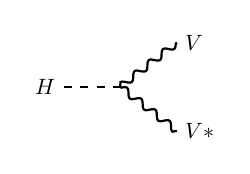
\begin{tikzpicture}[thick,scale=0.4,every node/.style={scale=0.8}]
  \begin{feynman}
    \coordinate[vertex] (v1);
    %\coordinate[vertex] (v2) at ($(v1)+(2,0)$));
    
    \coordinate[label=right :$V$] (q1) at ($ (v1) + (1.8,1.4) $);
    \coordinate[label=right :$V*$] (q2) at ($ (v1) + (1.8,-1.4) $);
    \coordinate[label=left :$H$] (h1) at ($ (v1) + (-1.8,0) $);
    \diagram* {
      (h1) -- [scalar] (v1),
      (q1) -- [boson] (v1)
      -- [boson] (q2),
    };
  \end{feynman}
\end{tikzpicture}


\end{document}
